\documentclass{article}
\usepackage{geometry}
% \usepackage{xeCJK}
\usepackage{amsmath}
\usepackage{amsthm}
\usepackage{indentfirst}
\usepackage{booktabs}
\usepackage{extarrows}
\usepackage{abstract}
\usepackage[dvipdfm]{graphicx}
\usepackage{cite}
\bibliographystyle{plain}
% \geometry{left=1cm,right=1cm,top=2cm,bottom=2cm}
\begin{document}
\author{519030910145 Qinwei Yang}
\title{\Huge{Quick-Hailer}\\\normalsize{A Smooth, Graceful and MultiFunctional APP for Analysis and Visualization of Online Ride-Hailing Order Data}}
\maketitle
\setcounter{tocdepth}{2}
\setlength{\parindent}{2em}

\section{Introduction}
Online car-hailing has opened up information communication channels for drivers and passengers. However, with the formation of Didi Taxi's monopoly, it has gradually been unable to keep up with the increasing functional and performance needs of users. 

In fact, the analysis of historical data can help us discover the temporal and spatial distribution patterns of the taxi supply and demand relationship, so as to achieve better dispatch.

Quick-Hailer can analyze the temporal and spatial distribution of order demand, duration, cost, and location, and provide route planning and itinerary estimation services.
\section{Implementation Details}
\subsection{Logical Structure}
\setlength{\parindent}{0em}
\begin{figure}[htbp] 
	\centering 
	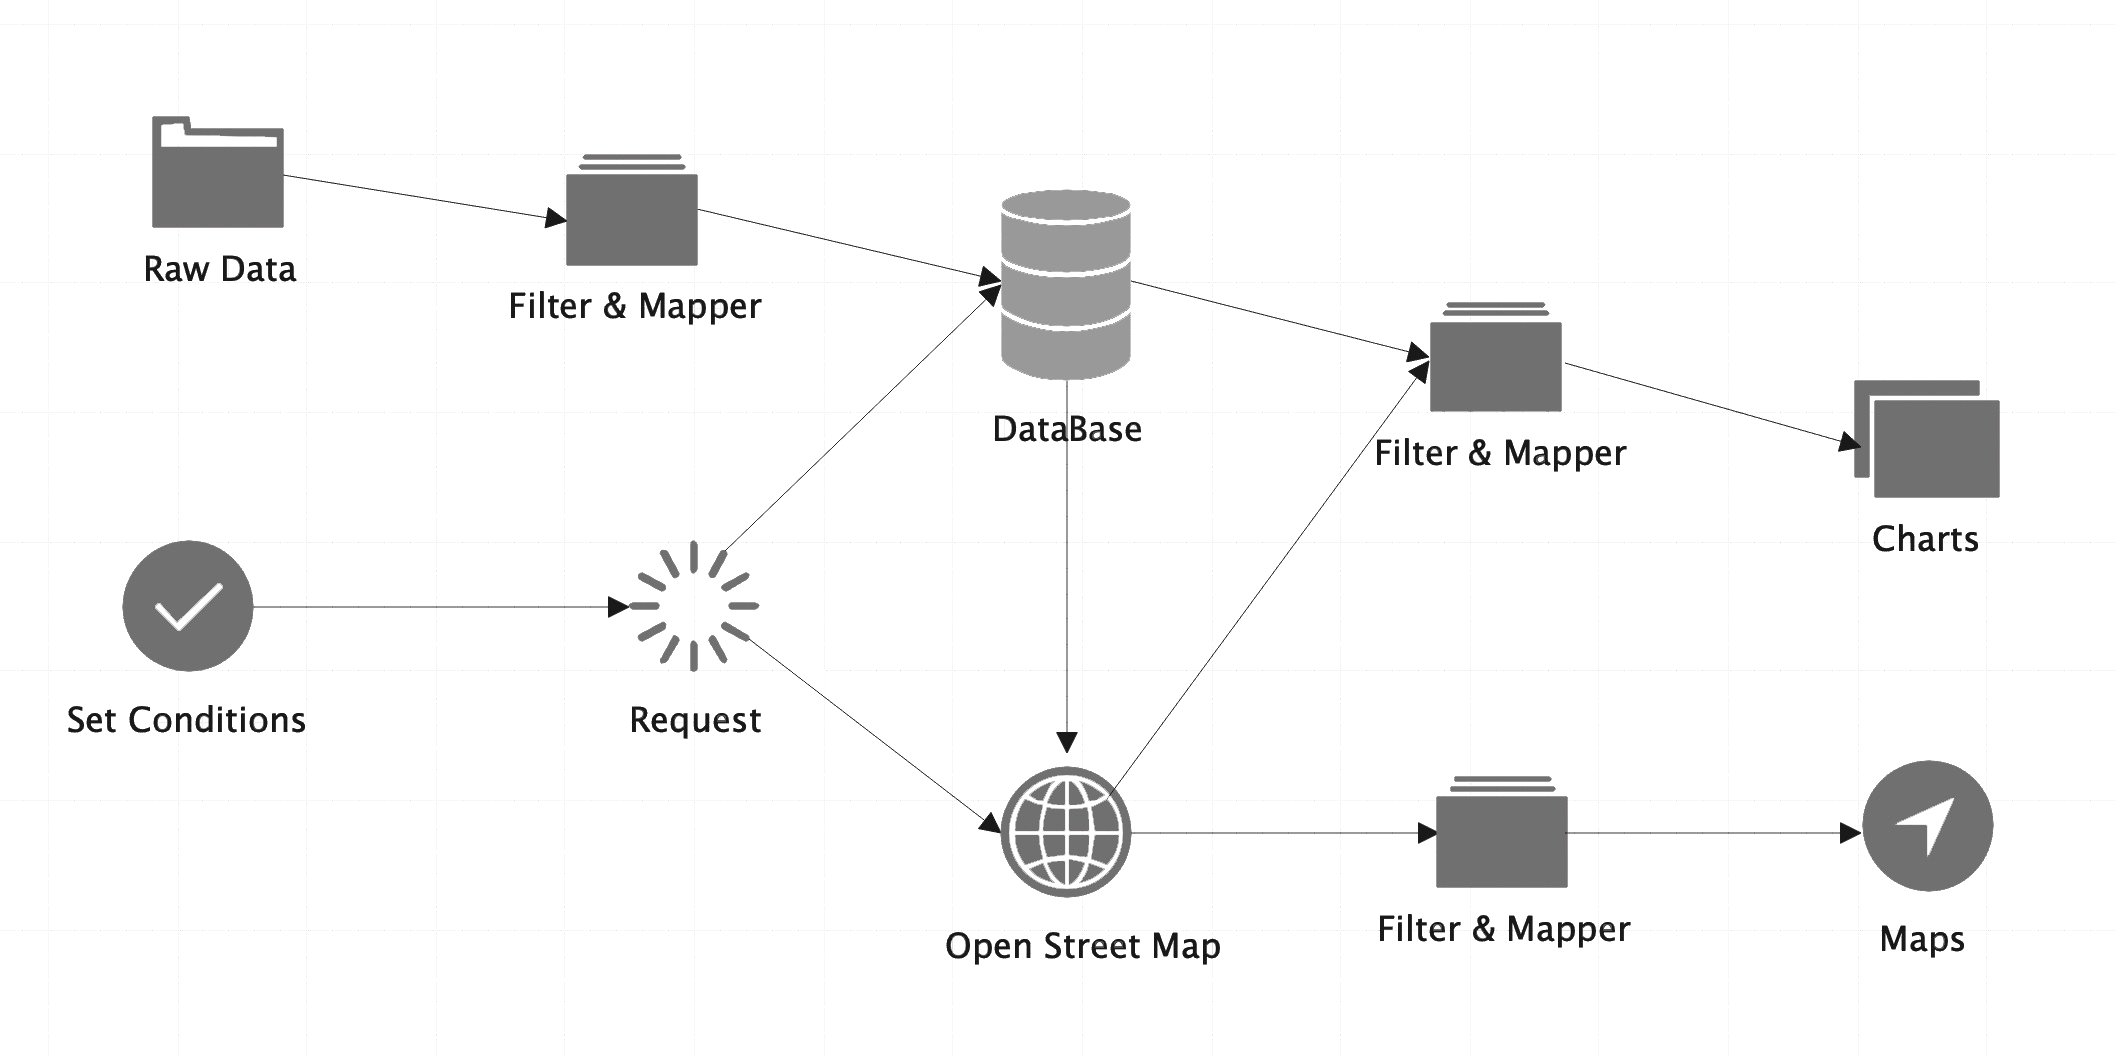
\includegraphics[scale=0.3]{LogicalStructure.png}
	\caption{Logical Structure Diagram}
\end{figure}
\setlength{\parindent}{2em}
As shown in the figure, all functions of Quick-hailer can be regarded as an act of searching, filtering, mapping, and rendering data.

Firstly, Quick-hailer uses a window to guide the user to select the original data and complete the first database load. In this process, you can select the field and time required by the user.

After setting the parameters, the user clicks the "Submit" button to send a request. The program will choose to extract data from the database or Open Street Map according to the type of request, and perform filtering and mapping.

Finally, the program renders the data to the corresponding chart or map.

In actual implementation, this logical model has the following points worth noting:
\begin{enumerate}
	\item Since each function has necessary requirements for some fields, only some fields are optional, and missing fields may cause some functions to be disabled.
	\item The operation in the logic model is performed in an additional thread, which will not affect the use of the main program. After the operation is completed, the status bar and loading animation will prompt the user.
	\item In order to prevent high-load requests to the database, the logic model will not work when other threads are currently performing data rendering.
	\item When 3 cannot be satisfied for some reason, the program will wait for other threads to complete the task before proceeding.
\end{enumerate}

\subsection{Program Structure}
\setlength{\parindent}{0em}
\begin{figure}[htbp] 
	\centering 
	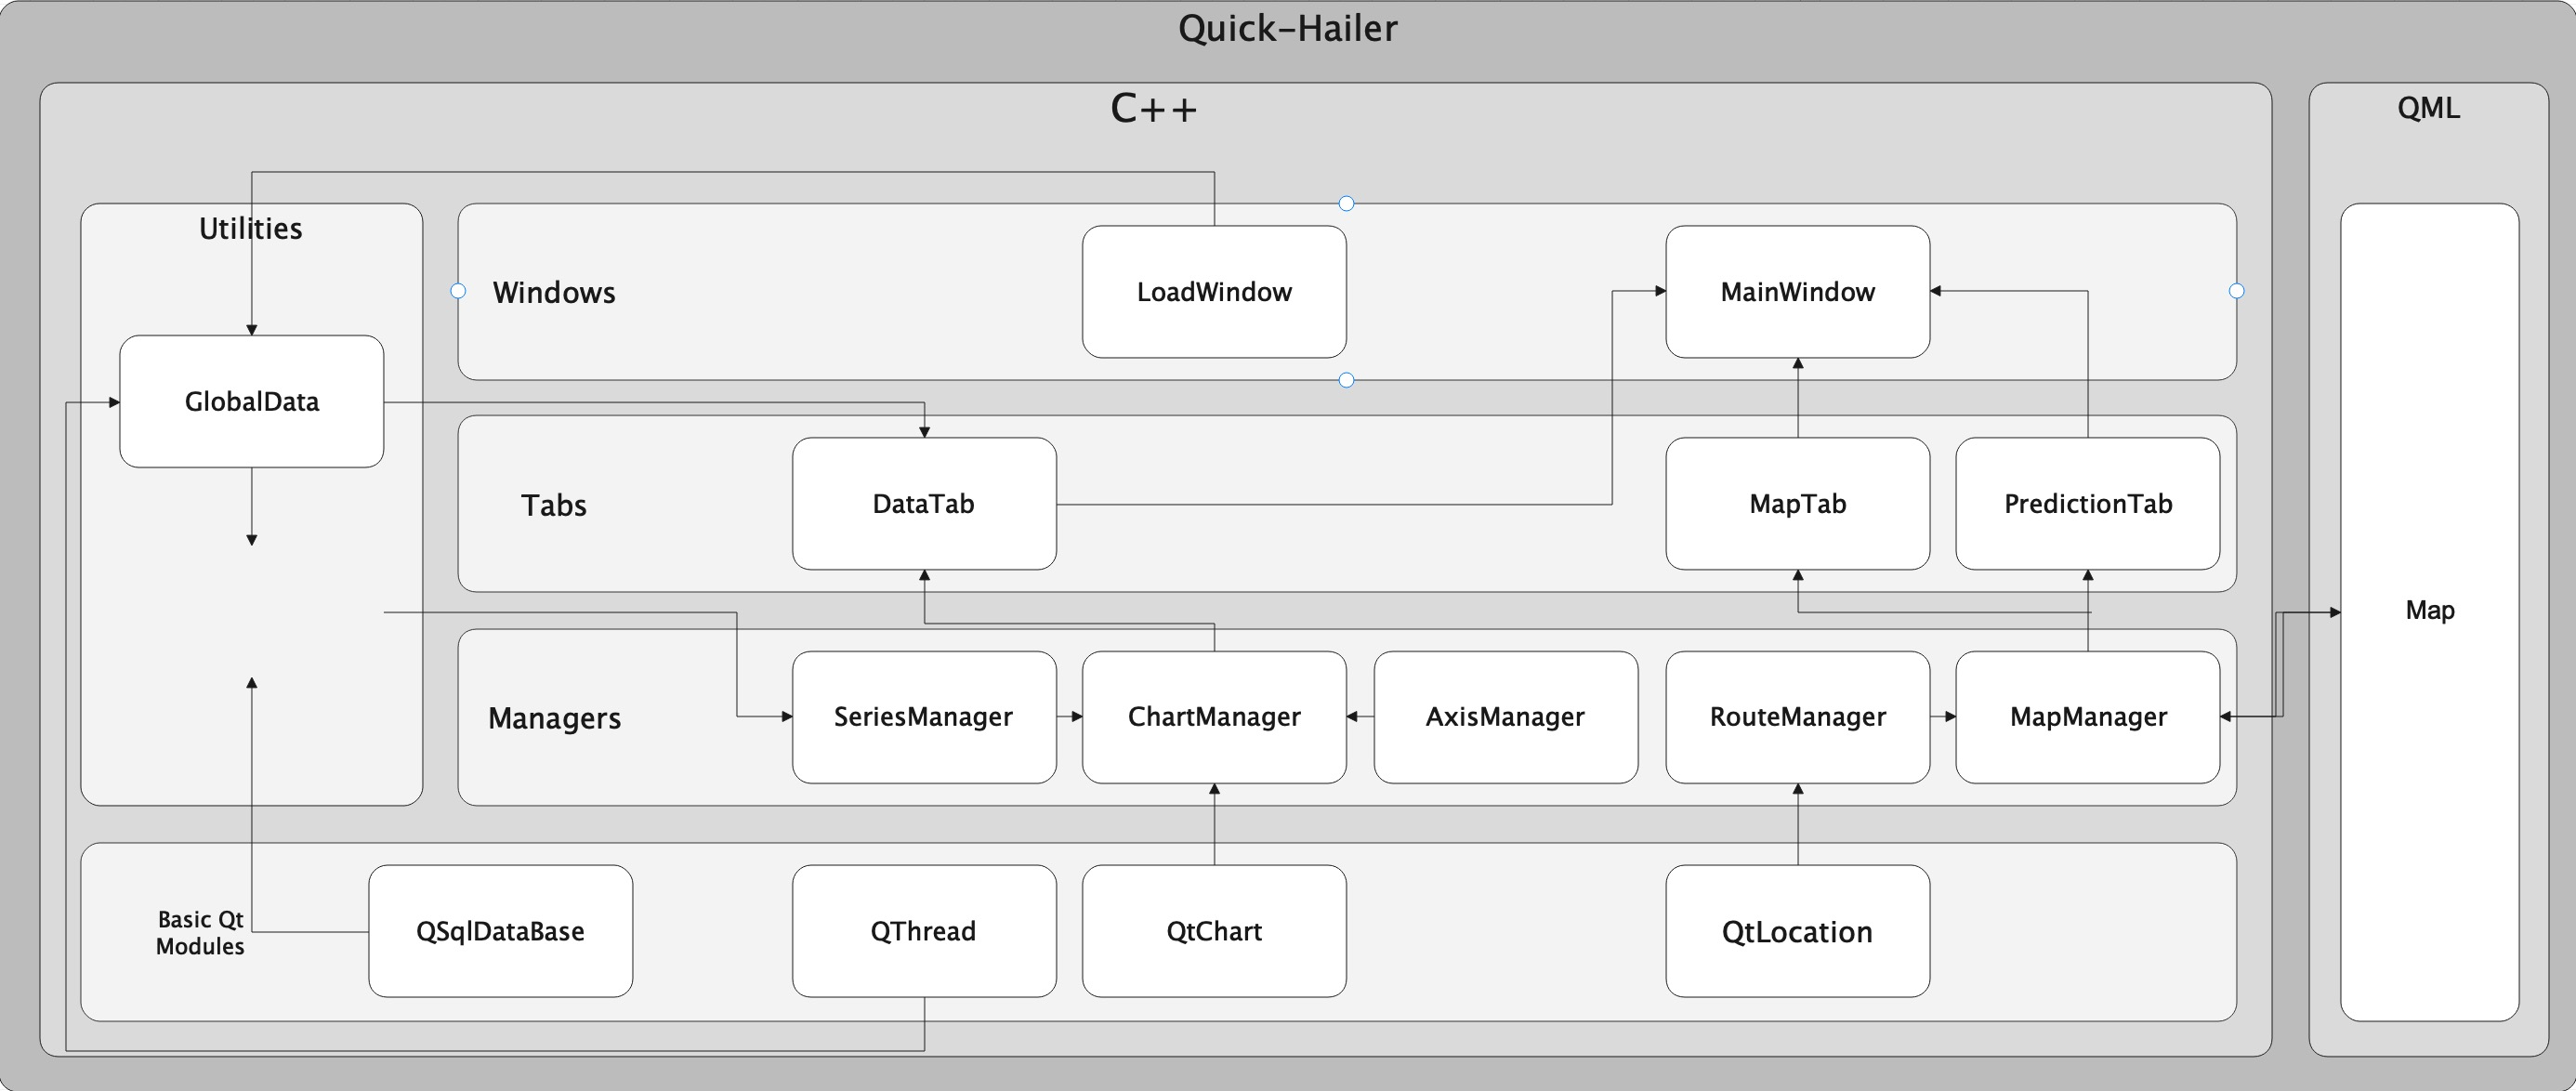
\includegraphics[scale=0.14]{ProgramStructure.png}
	\caption{Program Structure Diagram}
\end{figure}
\setlength{\parindent}{2em}
Quick-Hailer adopts the idea of ​​object-oriented programming, encapsulates some basic operations into five Managers, puts the signals/slots corresponding to windows and tabs into corresponding Windows/Tabs classes, and packs information and functions that needs to be used across files into a static instance of the Utilities class. Thereby enhancing its readability, maintainability and scalability.

It is worth mentioning that the communication between C++ and QML in Qt is very troublesome. In order to reduce unnecessary difficulties, Quick-Hailer uses MapManager as the registered class in the QML code, and declares the corresponding instance in the map file, and transmits data with the registered properties through the signal \& slot mechanism.

\setlength{\parindent}{0em}
\begin{figure}[htbp] 
	\centering 
	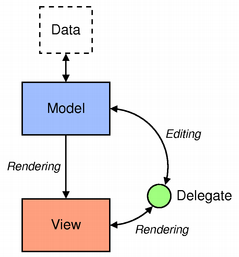
\includegraphics[scale=0.4]{modelview.png}
	\caption{MVC in QML}
\end{figure}
\setlength{\parindent}{2em}

To facilitate the rendering of large quantities of primitive data in QML maps, Quick-Hailer adopts the MVC design pattern. After setting up listModel and delegate in QML, we only need to pass in QVariantList from C++ as an object array, and we can load the map data.
\subsection{Data Processing}
The Quick-Hailer data set is very large, with 400,000 data records in just one day. If you store and maintain it directly in the program, it will not only be slow, but will also consume a huge amount of memory (about 2.5GB according to the test). Therefore, it is necessary to use a database.

The next question is how to access the database to obtain information. I thought of two methods:

A kind of intensive query, first obtain a large number of access requests through conditions, and then send these requests together, and finally the amount of data to be processed will be relatively small.

The other requires intensive filtering processing. The required data is extracted with one visit, and then the hash table is used for filtering and summarizing. In this way, all required records will be accessed sequentially during the processing.

Due to my unfamiliarity with the database, I cannot directly use SQL commands to obtain information in the first method, nor can I access it concurrently. This makes me actually still need to access all records sequentially and require more table lookup times and More indexes. Although increasing the index can increase the search speed, it will slow down the import speed. So I finally adopted the second method.

But I believe that if SQL can obtain the required information in one step and send requests concurrently, the speed of Quick-Hailer processing 15 days of information will be at least hundreds of times faster.
\subsection{User-friendly Features}
In addition, Quick-Hailer also implements some user-friendly small functions, such as:
\begin{enumerate}
	\item When analyzing the time distribution of taxi demand, you can visually select the required grids, and you can select all/unselect all with one click.
	\item When analyzing the heat map, the user can switch the analysis of the entire time period or a certain time point with one key.
	\item The analysis results of heat map and Taxi stream can be played to achieve the effect similar to GIF animation.
	\item In the route planning and prediction function, you can click on the map to pick up a point, and Quick-Hailer will analyze and display the address it points to.
	\item In the route planning function, the length of the road and the required time will be displayed every two steps.
\end{enumerate}
\section{Results}
\subsection{Overall characteristics}

\setlength{\parindent}{0em}
\begin{figure}[htbp] 
	\centering 
	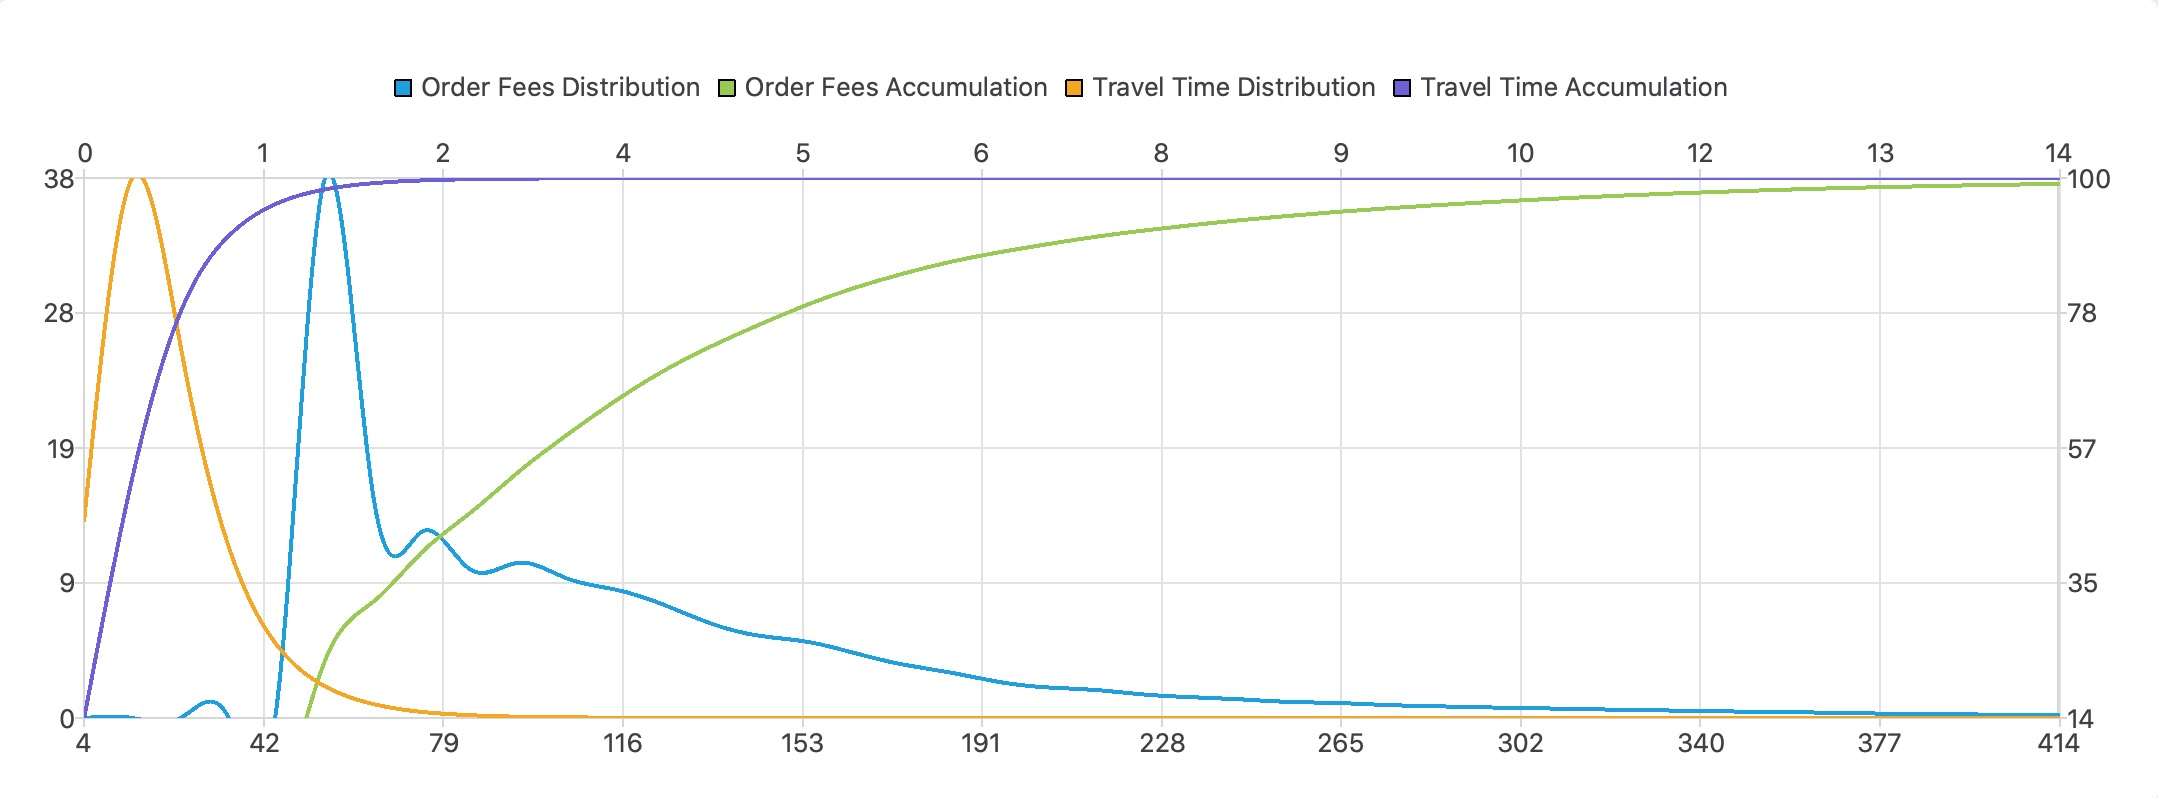
\includegraphics[scale=0.15]{all_distribution.jpg}
	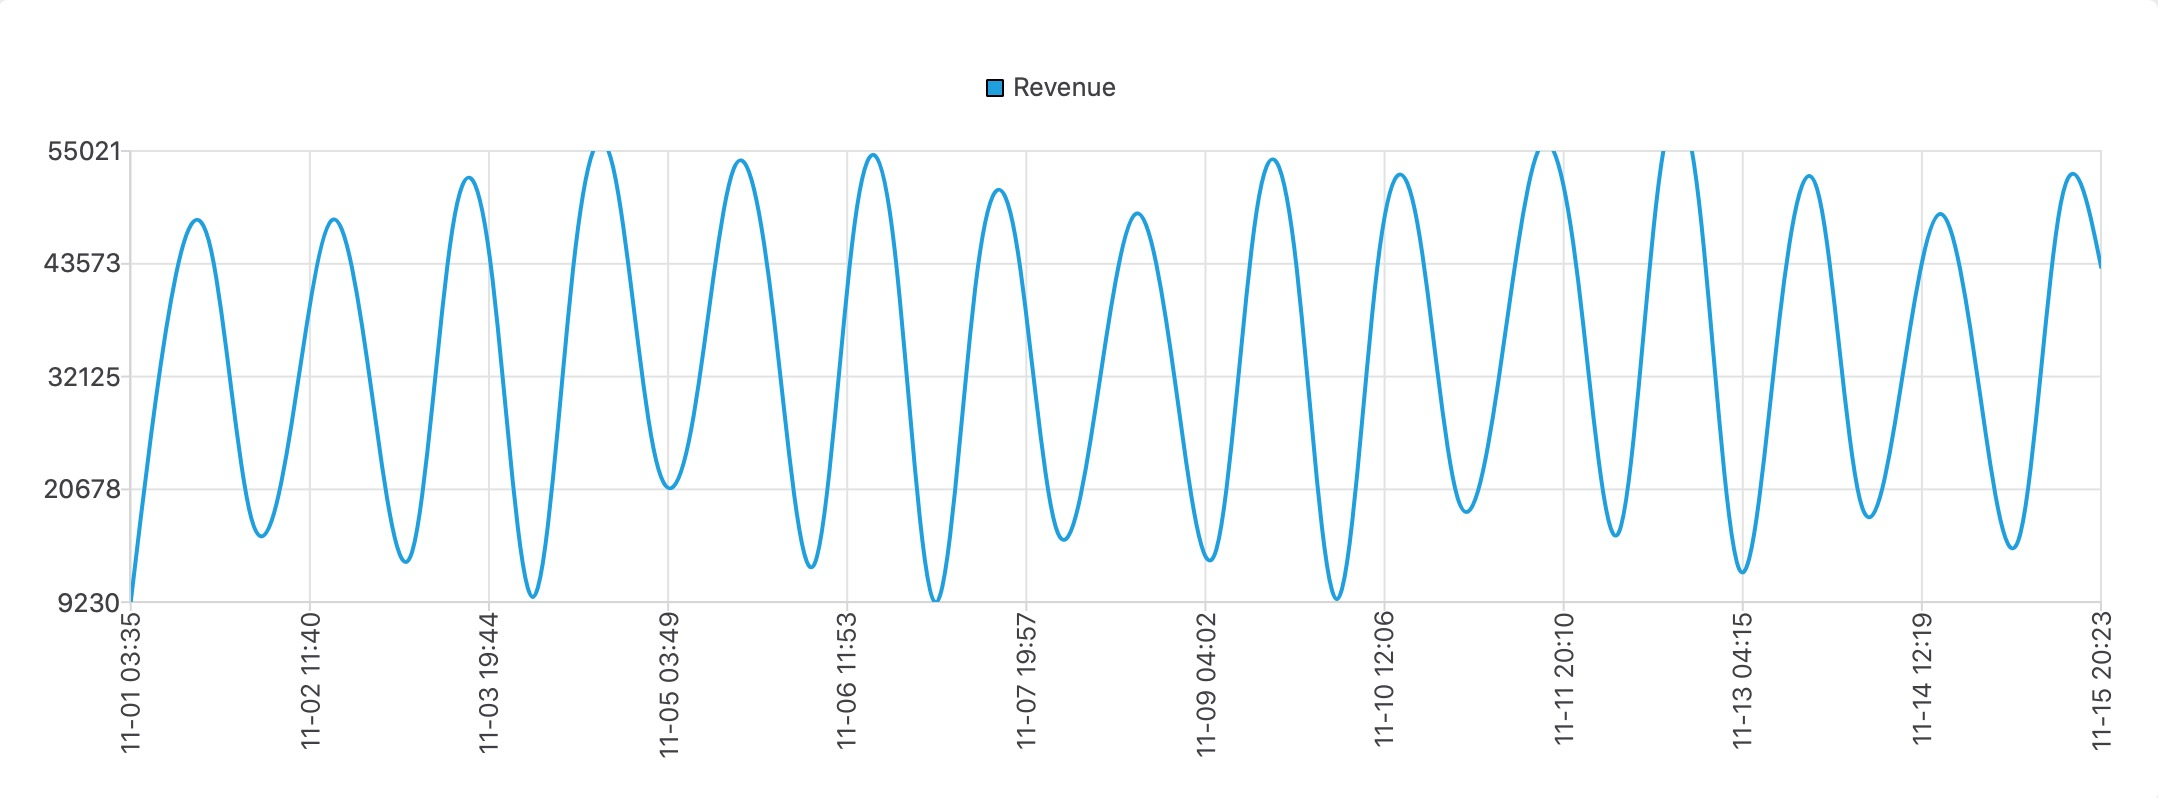
\includegraphics[scale=0.15]{new_all_revenue.jpg}
	\caption{Distribution \& Revenue}
\end{figure}
\setlength{\parindent}{2em}

We first observe the overall order duration and cost distribution, we can find that the order duration is mainly about 20 minutes, most of which are in the interval of 0-40 minutes, and only a few orders exceed 80 minutes; the order cost is between 1-2 yuan at most , And most of the rest are in the range of 2-10 yuan.

After observing the overall revenue curve, we can see that the total revenue of taxis changes periodically in a day-to-day cycle, while the daily peak and valley values ​​change periodically in a week-to-day cycle.

\subsection{Peak phenomenon}

\setlength{\parindent}{0em}
\begin{figure}[htbp] 
	\centering 
	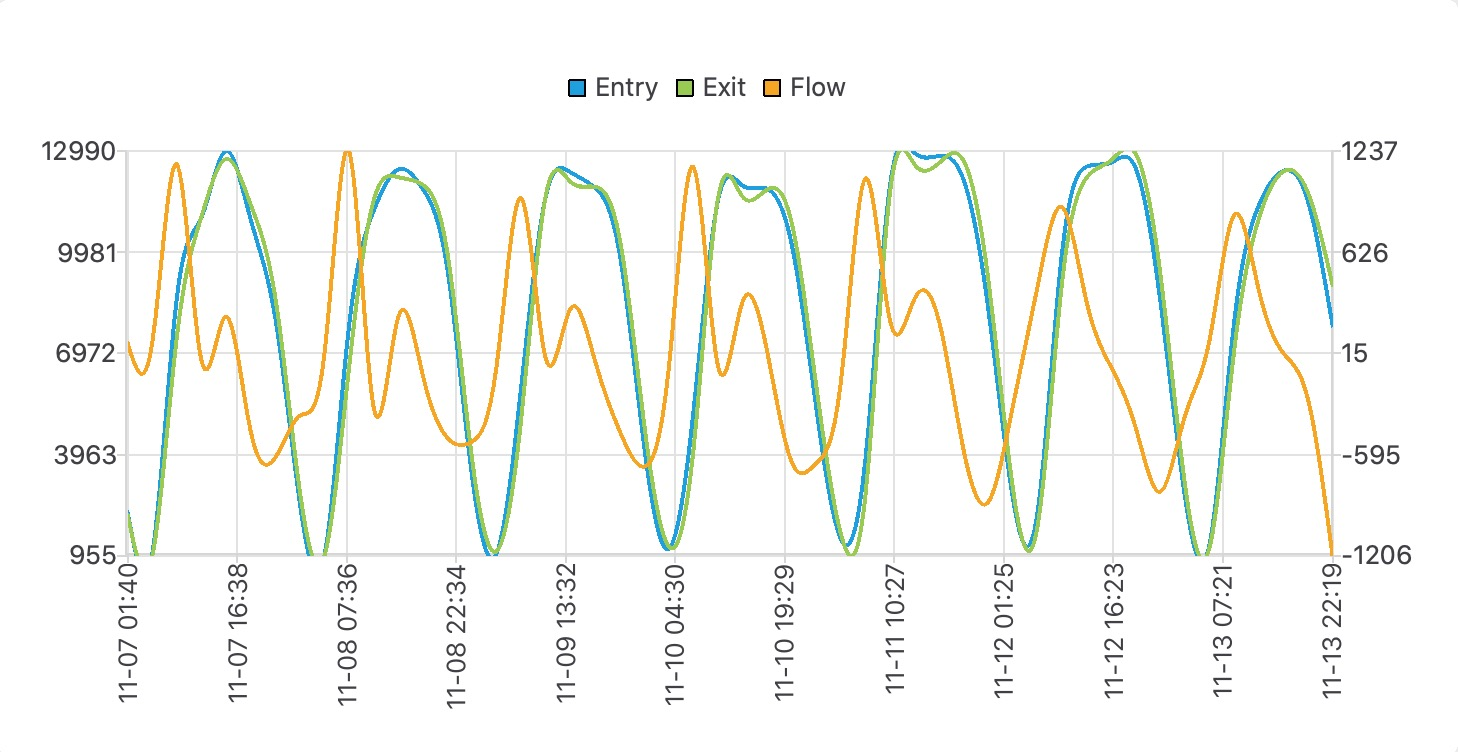
\includegraphics[scale=0.25]{new_week_demand.jpg}
	\caption{Week Demand}
\end{figure}
\setlength{\parindent}{2em}

We first observe the demand curve for the week from November 7th to 13th, and we can find that weekdays and weekends show significantly different distributions. This is in line with our common sense of life and is worthy of in-depth study.

\setlength{\parindent}{0em}
\begin{figure}[htbp] 
	\centering 
	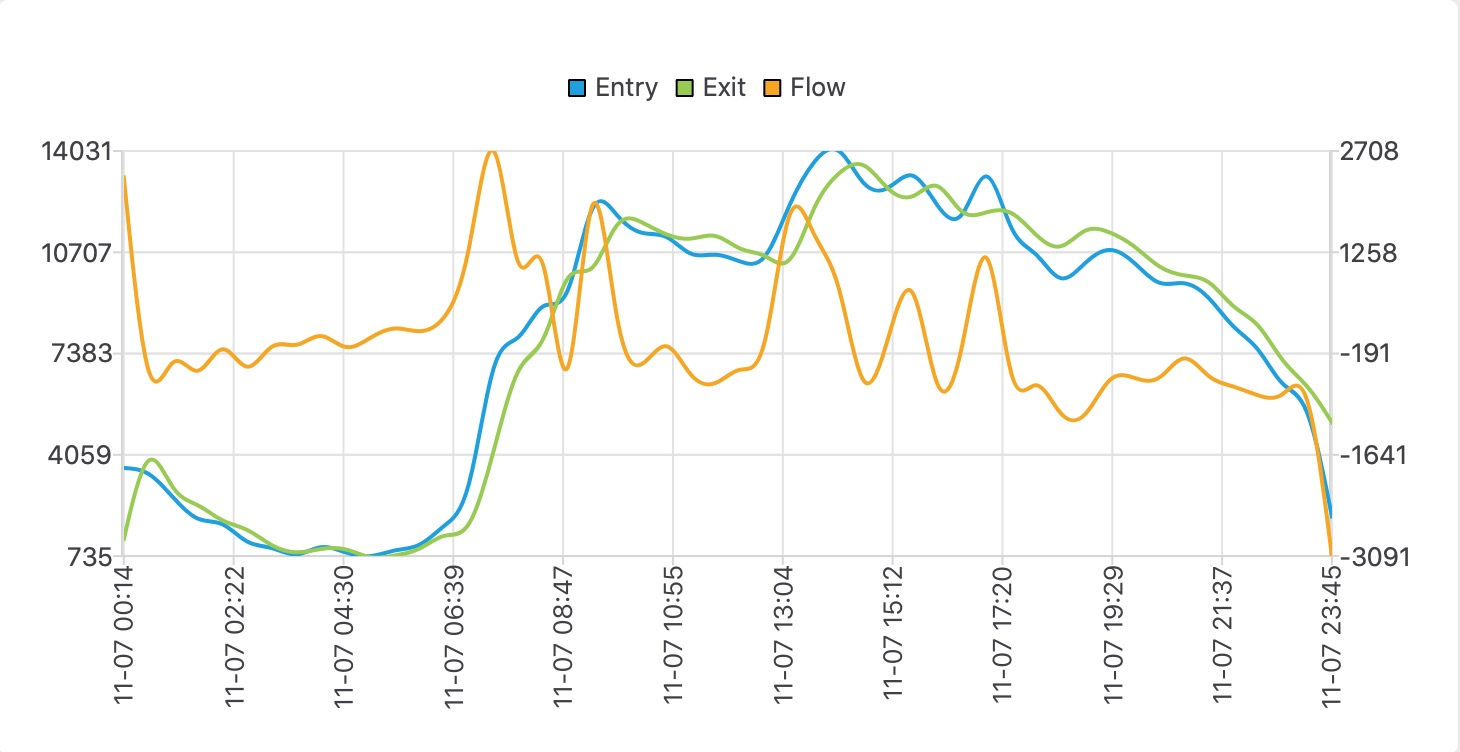
\includegraphics[scale=0.14]{new_daily_07_demand.jpg}
	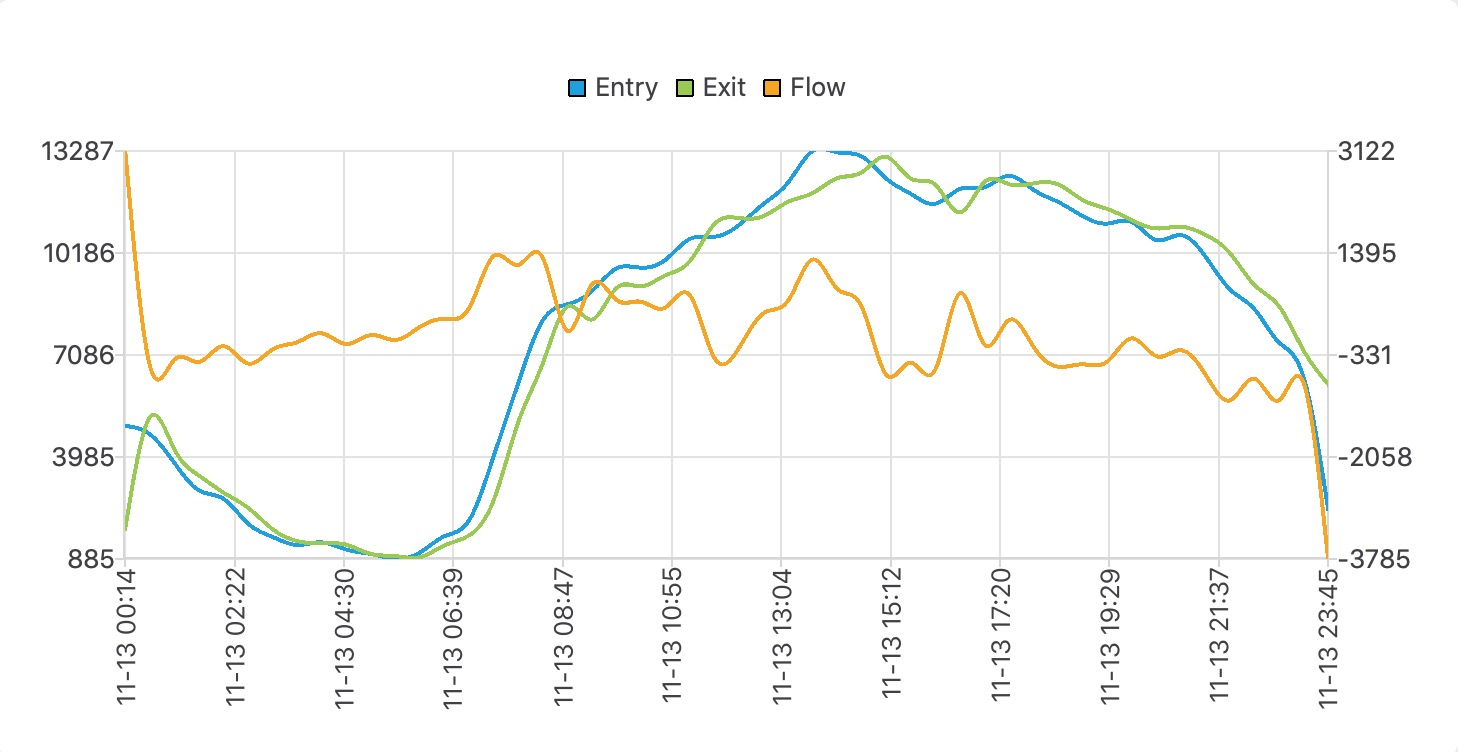
\includegraphics[scale=0.14]{new_daily_13_demand.jpg}
	\caption{Weekday \& Weekend}
\end{figure}
\setlength{\parindent}{2em}

Next, take November 7th and 13th as representatives to analyze the difference in demand patterns between weekdays and weekends. As shown in the figure, the demand curve on November 7 has 5 peaks, corresponding to the morning peak, the aftermath of the morning peak, lunch, afternoon tea, and dinner time, while the demand curve on the 13th is much smoother, with only a small peak during lunch time.

\setlength{\parindent}{0em}
\begin{figure}[htbp] 
	\centering 
	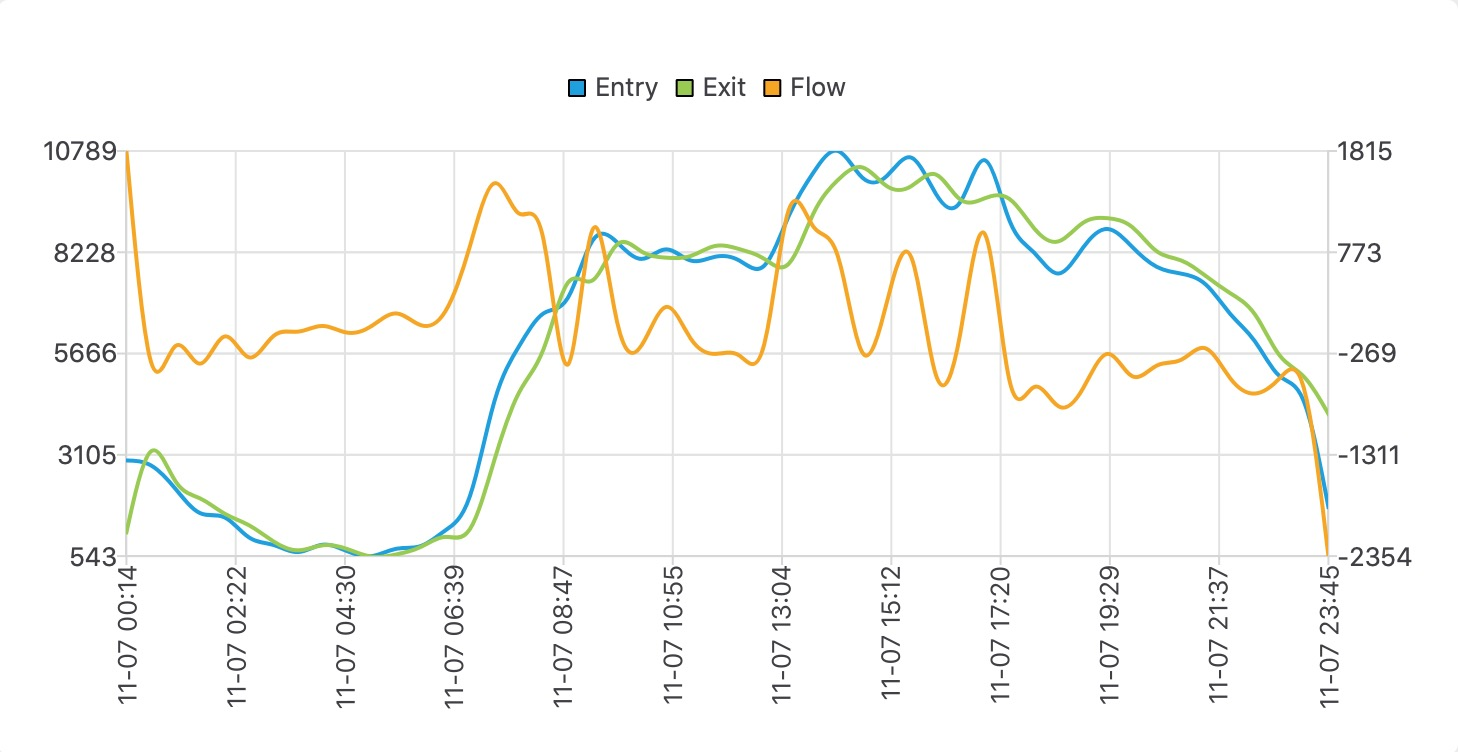
\includegraphics[scale=0.14]{new_city_07_demand.jpg}
	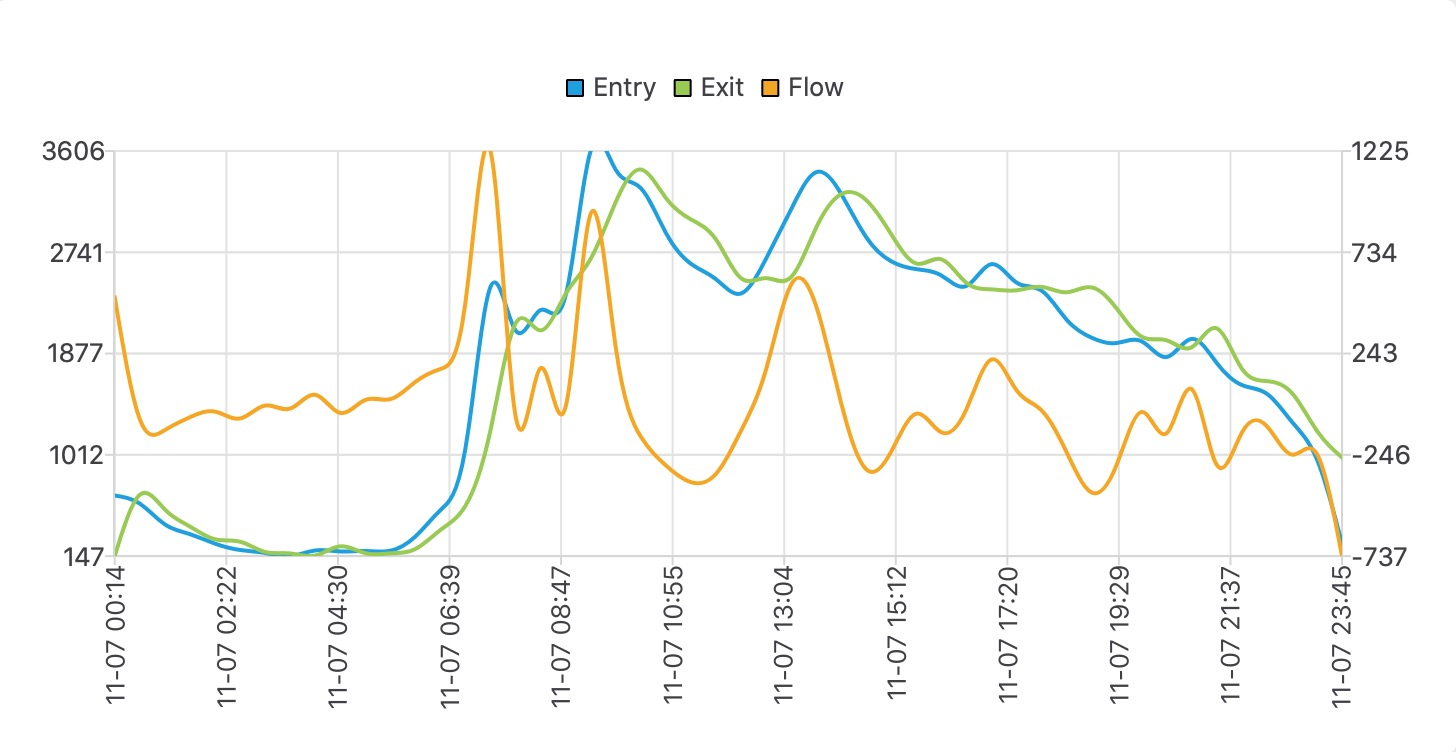
\includegraphics[scale=0.14]{new_town_07_demand.jpg}
	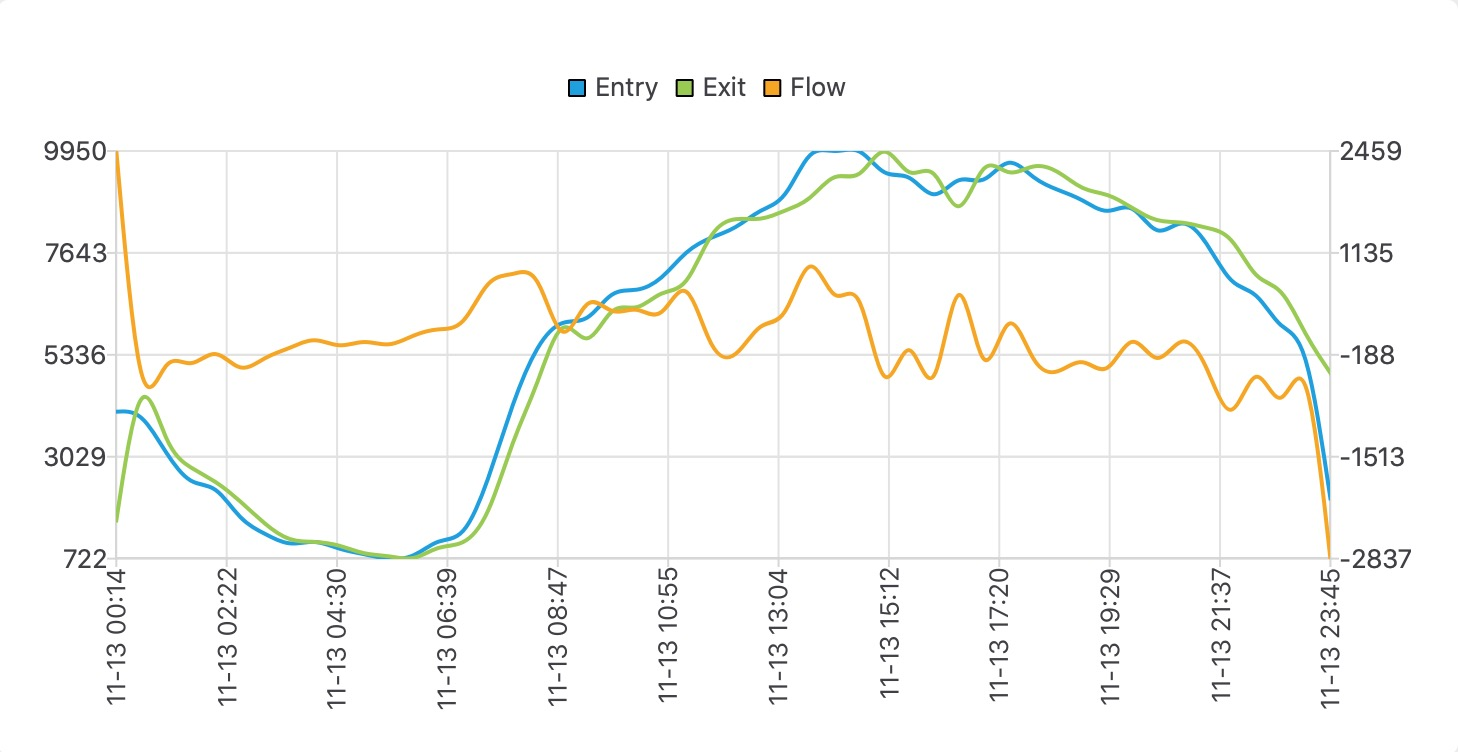
\includegraphics[scale=0.14]{new_city_13_demand.jpg}
	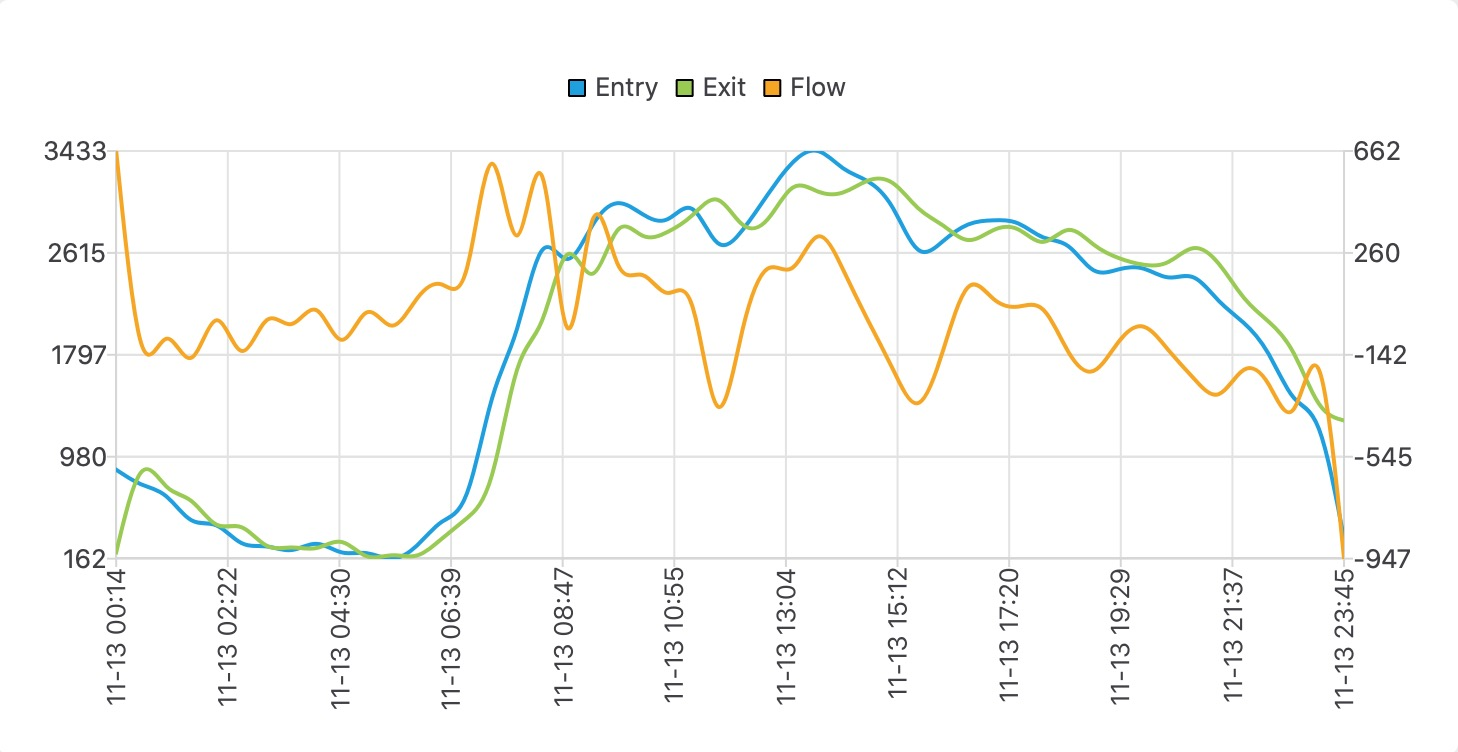
\includegraphics[scale=0.14]{new_town_13_demand.jpg}
	\caption{City \& Suburbs}
\end{figure}
\setlength{\parindent}{2em}

On the left is the urban area, on the right is the suburbs, the top ones is weekdays, and the bottom ones is weekends. In order to confirm our conjecture, we can observe the urban and suburban demand curves on the 7th and 13th. The figure shows that the morning and evening peaks in the suburbs are obviously stronger than that in the urban areas, and the obvious peaks can still be seen in the suburbs on weekends.

\subsection{Flow between urban and suburban areas}
\setlength{\parindent}{0em}
\begin{figure}[htbp] 
	\centering 
	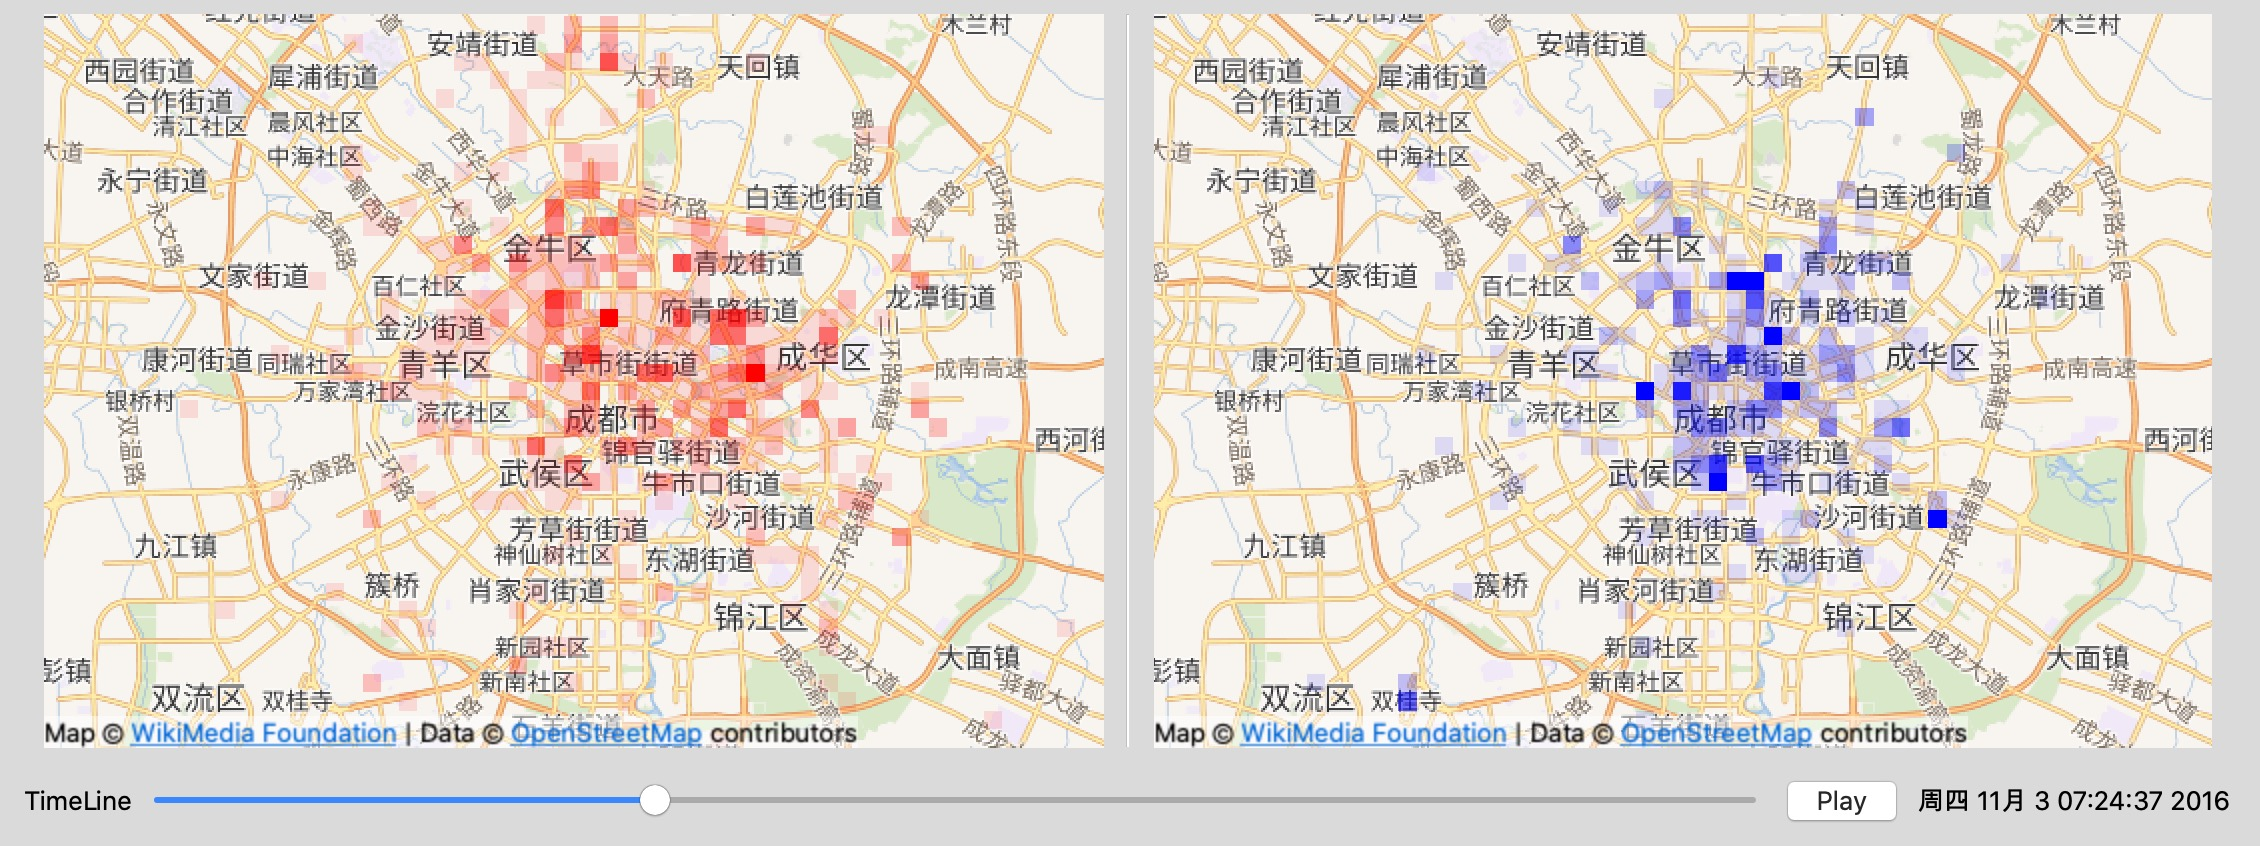
\includegraphics[scale=0.09]{morning.jpg}
	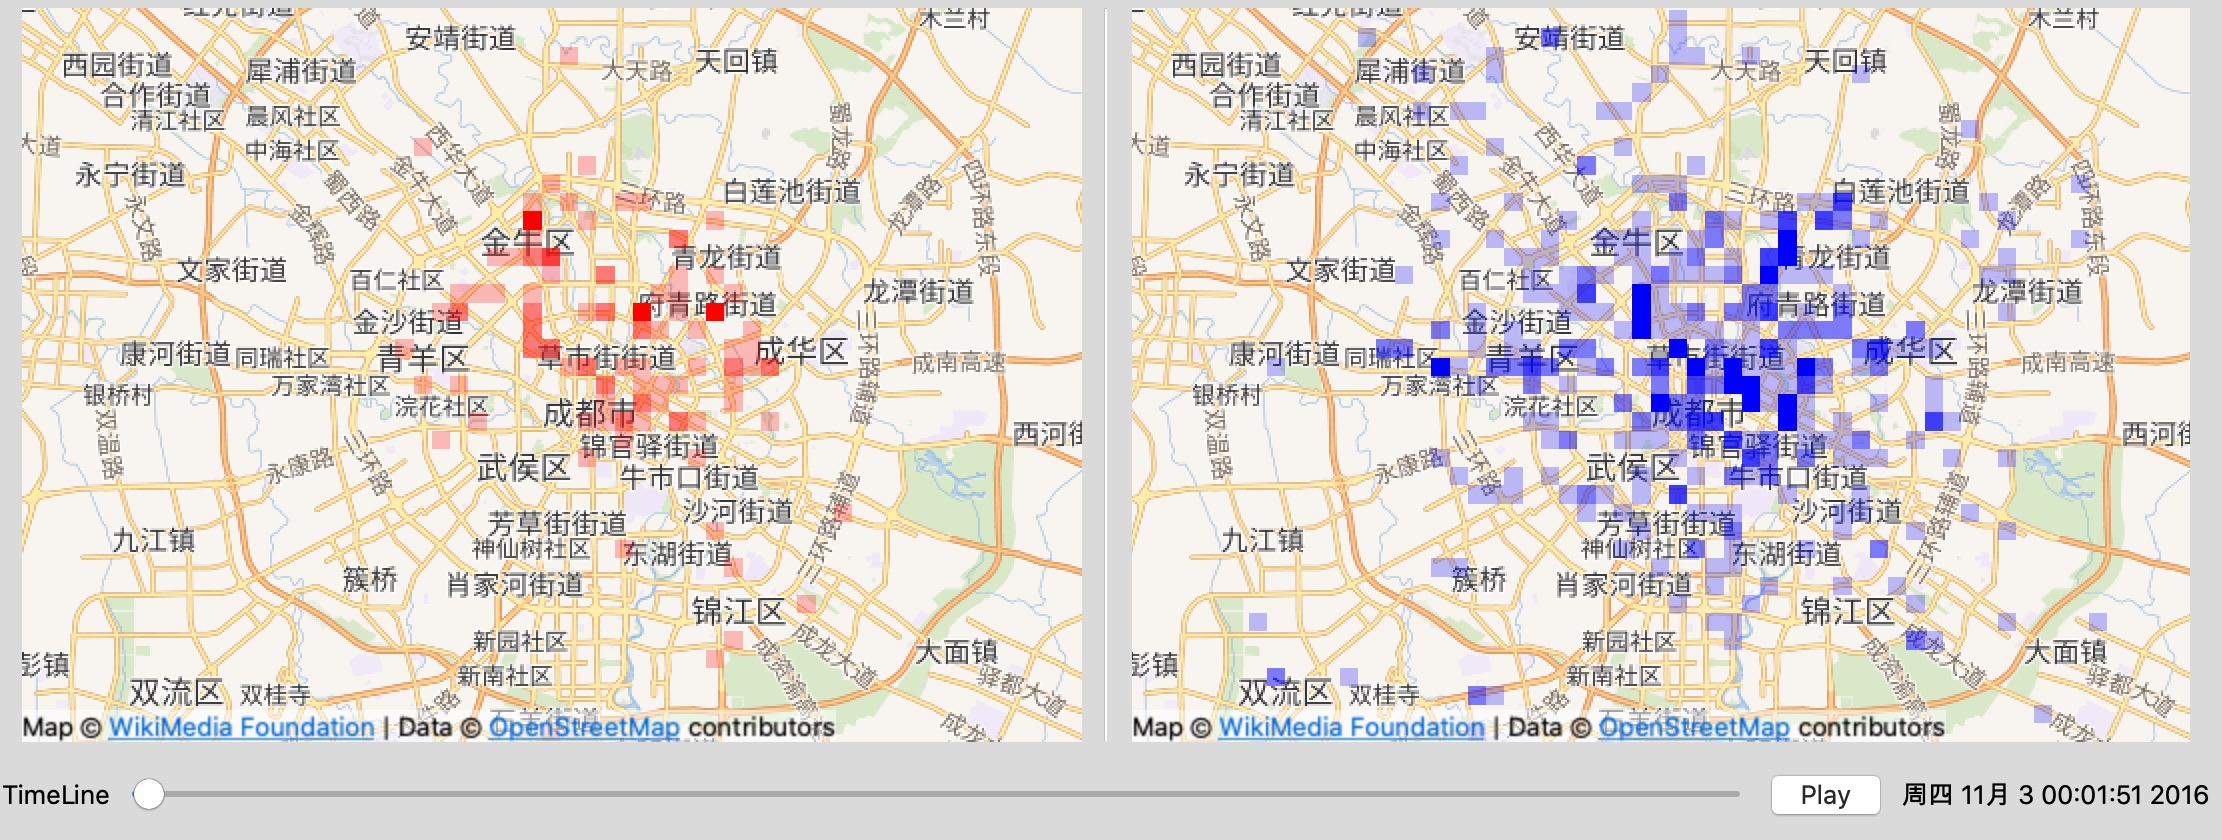
\includegraphics[scale=0.09]{night.jpg}
	\caption{Morning \& Night}
\end{figure}
\setlength{\parindent}{2em}
In the picture, red indicates the departure order, and blue indicates the din for getting off the bus. It can be seen from the figure that in the morning peak hours, a large number of people enter the city from the suburbs; at night, a large number of people travel from the city to the suburbs.

\newpage

\setlength{\parindent}{0em}
\begin{figure}[htbp] 
	\centering 
	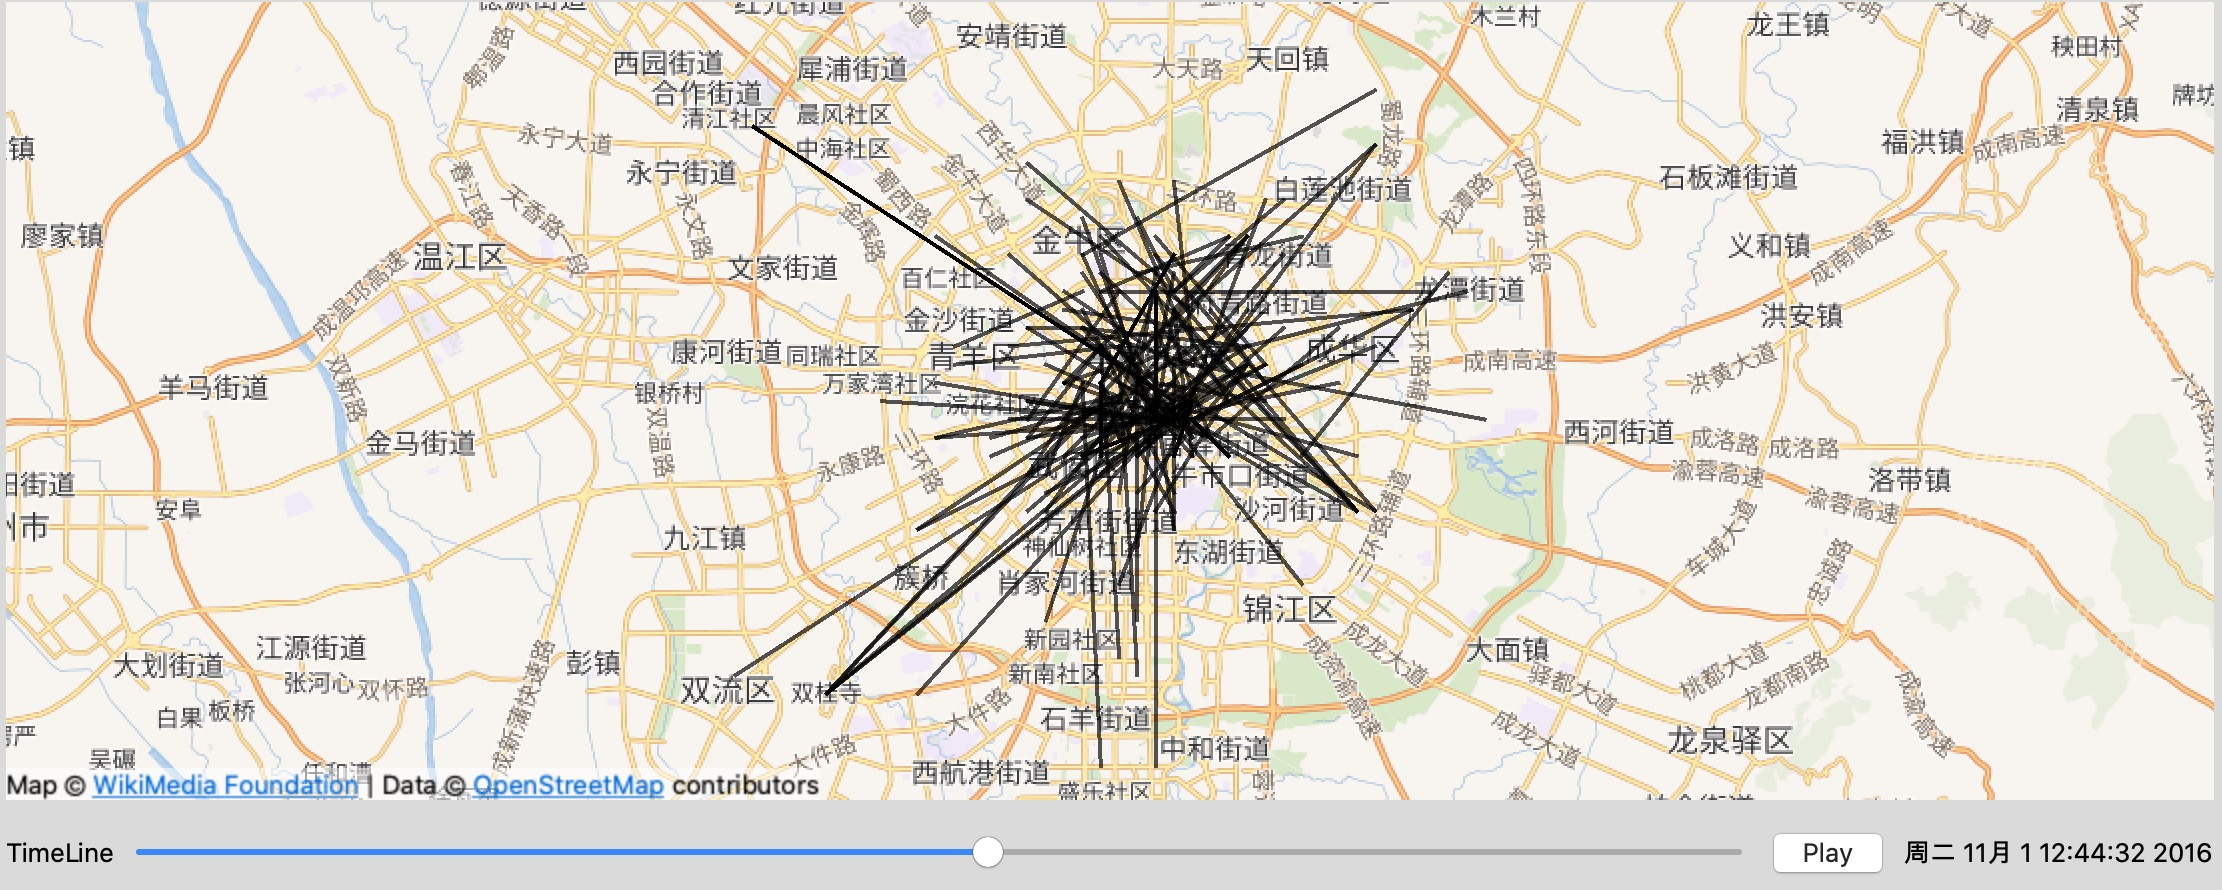
\includegraphics[scale=0.14]{flow.jpg}
	\caption{City \& Suburbs}
\end{figure}
\setlength{\parindent}{2em}

Examining the connection between the starting point and the ending point, we can find that some peripheral streets are closely connected with the city center, especially the streets in the south and northeast. At the same time, the vicinity of Shuanggui Temple is a large population distribution center because there is an airport there.

\subsection{About the airport}
\setlength{\parindent}{0em}
\begin{figure}[htbp] 
	\centering 
	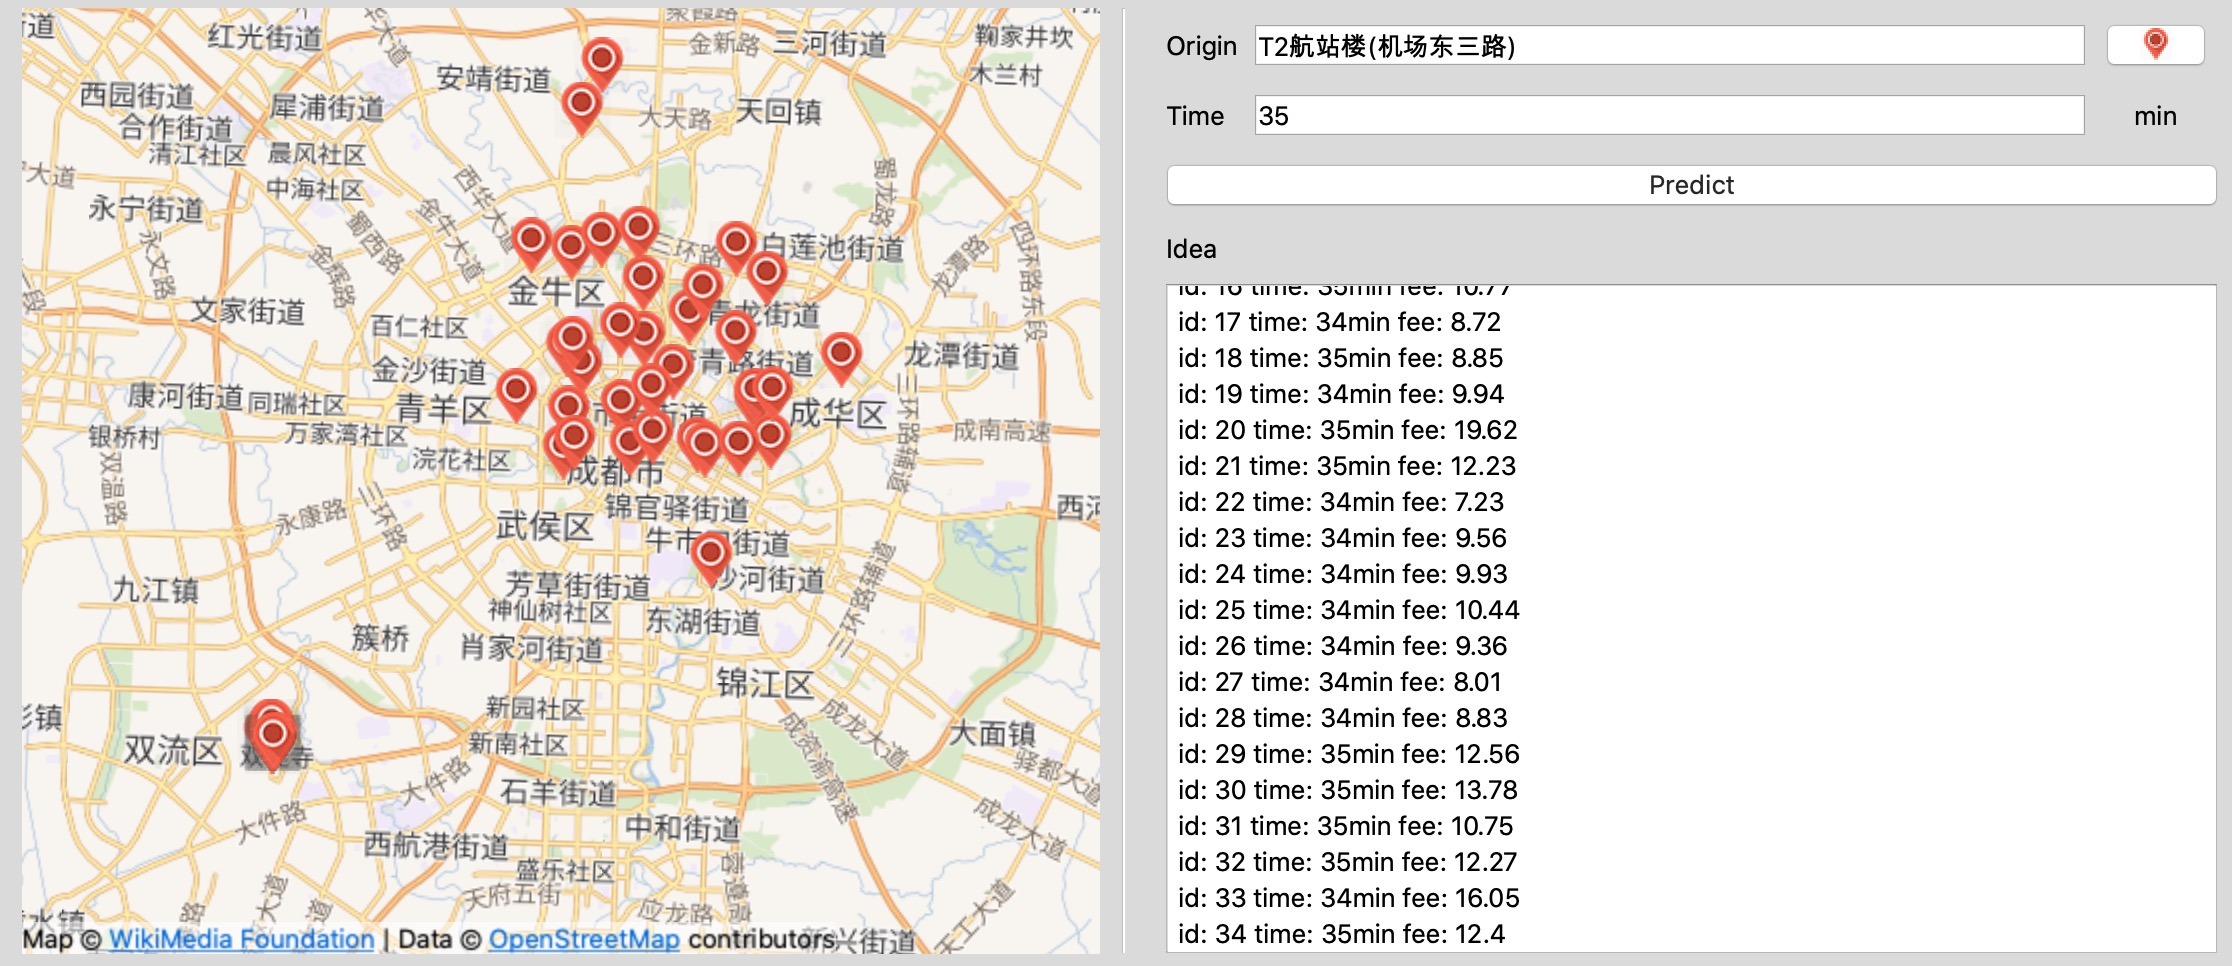
\includegraphics[scale=0.14]{realPlane.jpg}
	\caption{Shuangliu Airport}
\end{figure}
\setlength{\parindent}{2em}
Using our location prediction function, it can be deduced that it takes only 30-40 minutes to reach Shuangliu Airport from the northeast of the city.
\section{Discussions}
\subsection{Performance}
The test environment is \emph{Macbook Pro 13inch, Mid 2020}, the CPU is a quad-core Intel Core i7, the main frequency is 2.3GHz, and the memory is 32GB 3733 MHz LPDDR4X. The network bandwidth used during the test is 400Mbps. 

\begin{table}[htbp]
	\centering
	\begin{tabular}{lc}
		\toprule
		Task	&	Average Time(s)	\\
		\midrule
		Load data (1 day)	&	2.31	\\
		Load data (15 days)	&	42.15	\\
		Render demand chart (1 day)	&	1.48	\\
		Render demand chart (15 days)	&	25.40	\\
		Render all charts (1 day)	&	6.16	\\
		Render all charts (15 days)	&	101.14	\\
		Render Overall Thermal Diagram (1 day)	&	2.05	\\
		Render Overall Thermal Diagram (15 days)	&	23.45	\\
		Route Planning	&	2.91	\\
		Route Based Prediction (15 days)	&	0.26	\\
		Space Based Prediction (15 days)	&	0.21	\\
		\bottomrule
	\end{tabular}
	\caption{Performance Test Result}
\end{table}

After loading all data sets, the storage space occupied by the program is 499kB, the storage space occupied by the database is 455MB, the memory consumption is 353.7MB, and the peak CPU consumption is 20\%, maintaining a good balance among various performances.

\subsection{Expand ideas}
In addition, I have some other thoughts about Quicker-Hailer. However, they have not been implemented due to time constraints:
\begin{enumerate}
	\item When rendering the connection between the start point and the end point of an order at a certain moment, I intended to show the path between them. However, because the current route planning function of Quicker-Hailer needs to access the online osm, there will be a high network delay when displaying, which conflicts with the function of play, and has to give up. Maybe I can configure an offline map library to solve this problem.
	\item The current function of rendering charts is not convenient enough. I am going to implement a function that can quickly select and browse a certain week, a certain day or a certain hour, and can be adjusted by sliding, just like the slider at the bottom of MapTab.
	\item The interactivity of charts is not enough. I can support the mouse and touchpad so that it can accept operations such as sliding, hovering, and zooming.
	\item The use of Space based prediction is too rigid, I can make it achieve an effect similar to drawing a layered and colored topographic map.
	\item As mentioned earlier, the way the database is used has yet to be optimized.
\end{enumerate}
\section{Acknowledgement}
Thanks to Dr. Ling and Dr. Jin for their careful teaching.

Thanks to JaredTao for his articles about Qt on Zhihu, which helped me a lot. 
\end{document}